\documentclass{sigchi}

\toappear{ Copyright \copyright 2015. edX. This document may be redistributed under the terms of the CC-BY-SA 3.0 or later, or AGPL v3.0 or later. \\
See: \textsc{https://creativecommons.org/licenses/by-sa/3.0/}\\
\textsc{http://www.gnu.org/licenses/agpl-3.0.en.html} for details.\\
{\emph{UIST'15}}, November 8-11, 2014, Charlotte, NC.}

% Load basic packages
\usepackage{balance}  % to better equalize the last page
\usepackage{graphics} % for EPS, load graphicx instead
\usepackage{times}    % comment if you want LaTeX's default font
\usepackage{url}      % llt: nicely formatted URLs

% llt: Define a global style for URLs, rather that the default one
\makeatletter
\def\url@leostyle{%
  \@ifundefined{selectfont}{\def\UrlFont{\sf}}{\def\UrlFont{\small\bf\ttfamily}}}
\makeatother
\urlstyle{leo}


% To make various LaTeX processors do the right thing with page size.
\def\pprw{8.5in}
\def\pprh{11in}
\special{papersize=\pprw,\pprh}
\setlength{\paperwidth}{\pprw}
\setlength{\paperheight}{\pprh}
\setlength{\pdfpagewidth}{\pprw}
\setlength{\pdfpageheight}{\pprh}

% Make sure hyperref comes last of your loaded packages, 
% to give it a fighting chance of not being over-written, 
% since its job is to redefine many LaTeX commands.
\usepackage[pdftex]{hyperref}
\hypersetup{
pdftitle={Collaborative Multimodal Annotation System for Peer Discussion at Scale},
pdfauthor={LaTeX},
pdfkeywords={SIGCHI, proceedings, archival format},
bookmarksnumbered,
pdfstartview={FitH},
colorlinks,
citecolor=black,
filecolor=black,
linkcolor=black,
urlcolor=black,
breaklinks=true,
}

% create a shortcut to typeset table headings
\newcommand\tabhead[1]{\small\textbf{#1}}


% End of preamble. Here it comes the document.
\begin{document}

\title{Multimodal Peer Discussion with RichReview on edX}

\numberofauthors{3}
\author{
  \alignauthor Dongwook Yoon\\
    \affaddr{Cornell University}\\
    \affaddr{Ithaca, NY 14850}\\
    \email{dy252@cornell.edu}\\
  \alignauthor Piotr Mitros\\
    \affaddr{edX}\\
    \affaddr{Cambridge, MA 02139}\\
    \email{pmitros@edx.org}\\
}

\maketitle

\begin{abstract}
Abstract
\end{abstract}

\keywords{
	Massive open online courses; peer discussion; multimodal annotation; voice user interface; peer group assignment.
}

\category {H.5.3.}{Group and Organization Interfaces}{Collaborative computing}[] 
\category {H.5.2.}{User Interfaces}{Interaction styles}[] 
\category {H.5.1.}{Multimedia Information Systems}{Audio input/output}[] 

\section{Introduction}

Peer-discussion in classrooms can improve student learning outcomes~\cite{chi2014icap}, in particula, strengthening students’ mental model about concepts~\cite{nicol2003peer} and broaden student perspectives on problem solving~\cite{smith2009peer}.
Massive open online course providers provide a large number of students with online peer discussion activities through discussion forums~\cite{13Mitros6002}, video chats, and peer feedback on assignments~\cite{linc}. These face a tradeoff between the richness of synchronous interaction and the flexibility of asynchronous interactions.

Recently, we presented a multimodal annotation system called RichReview~\cite{yoon2014richreview}.
RichReview brings expressivity into asynchronous document annotations through the use of student-recorded multimedia, including text, audio, and gestures.
The system was built for purpose of writing feedback, but was designed to supporting a range of modes of online peer-discussion.

In this work, we demonstrate how integration of RichReview into a MOOC platform can potentially open an expressive discussion channel among a large number of students.
As the first step, we re-implemented the RichReview's front-end, integrating it into Open edX. We designed a scalable back-end architecture for transmitting and storing multimedia comments created by a number of students.
We partner these with a novel peer-group assignment scheme that maximizes overall diversity of group composition using student profile data.

\begin{figure}[!h]
\centering
{
\setlength{\fboxsep}{0pt}
\setlength{\fboxrule}{0.5pt}
\fbox{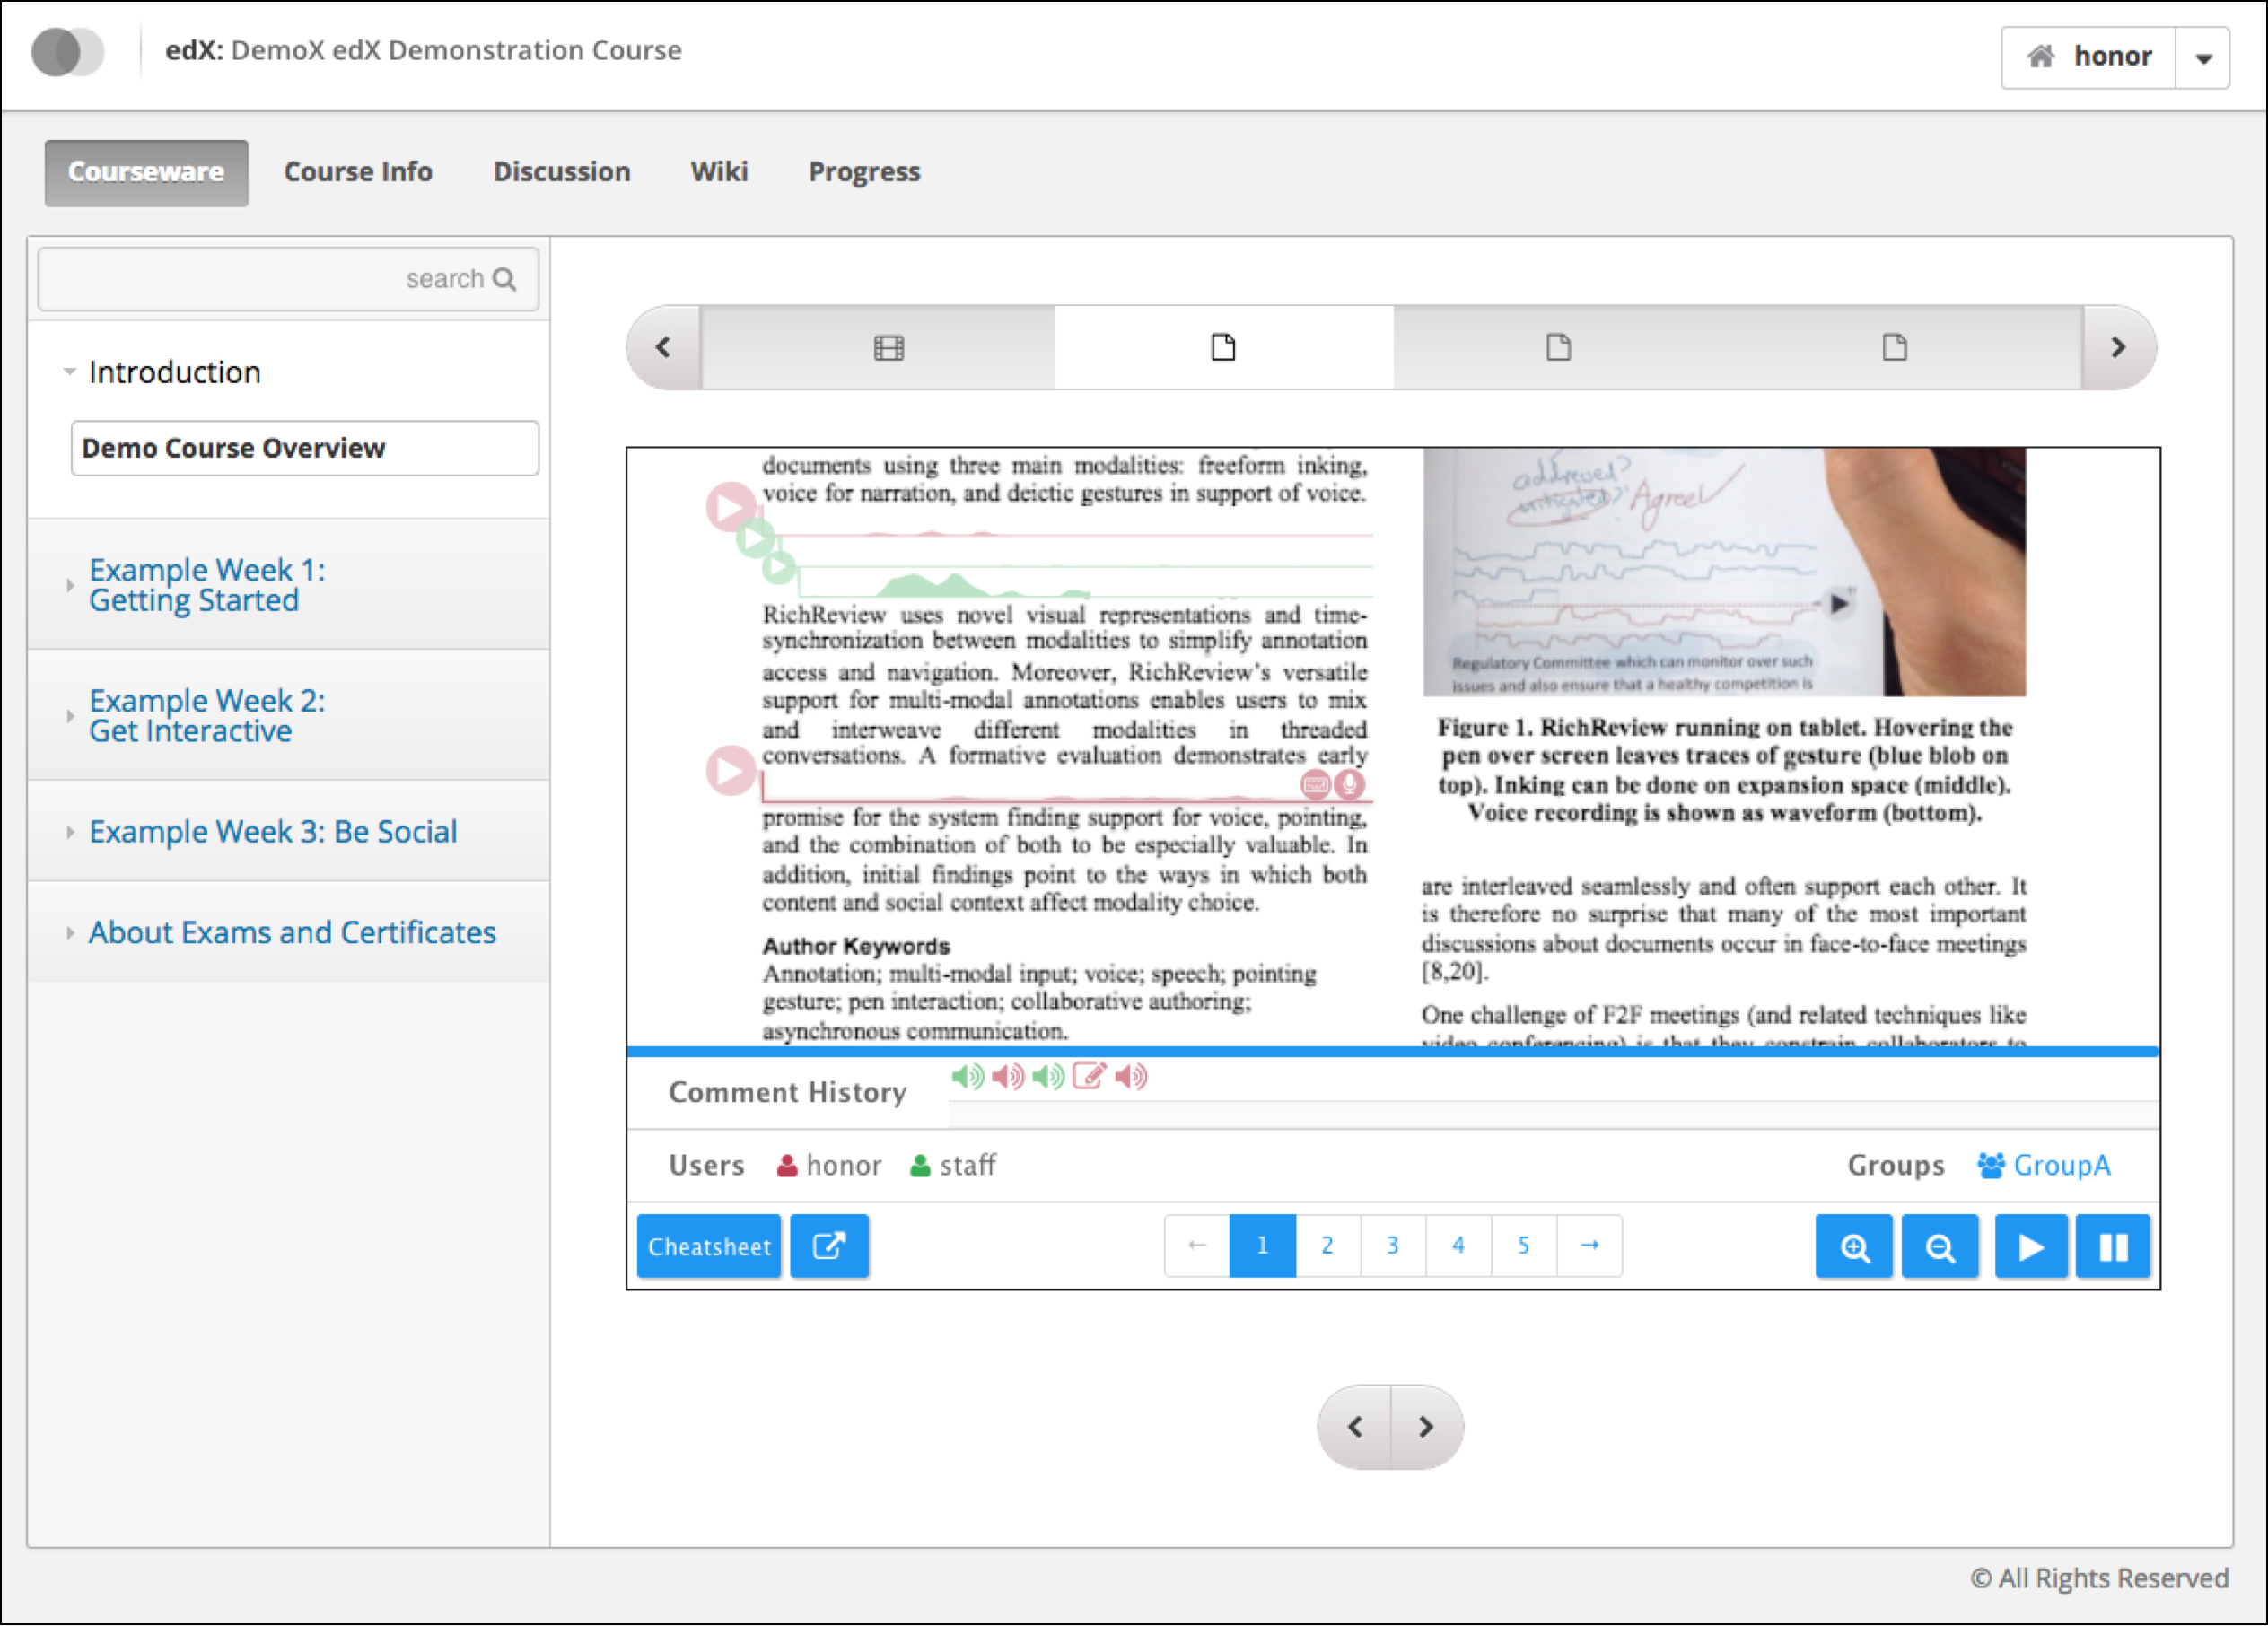
\includegraphics[width=0.95\columnwidth]{figure_edx}}
}
\caption{The RichReview web applet running in the edX courseware.}
\label{fig:screenshot}
\end{figure}


\section{RichReview Multimodal Annotation System}
RichReview is a tablet based multimodal annotation system for bringing richness of in-person conversation into document writing revision process.
With RichReview, a commentator can record a combination of input modalities, such as pen writing and hovering, voice recording, as well as traditional modalities such as text.
For example, RichReview users can verbally explain a math concept while pointing to a relevant formula in a document and drawing a graph.
Moreover, RichReview embeds the annotation thread within text lines of the annotated document, giving clear context for the comments.
A prior lab study promised potential of the rich commenting system as a supporting tool for document-centric conversation~\cite{you-know-this-one-better-than-i-do}.

\begin{figure}[!h]
\centering
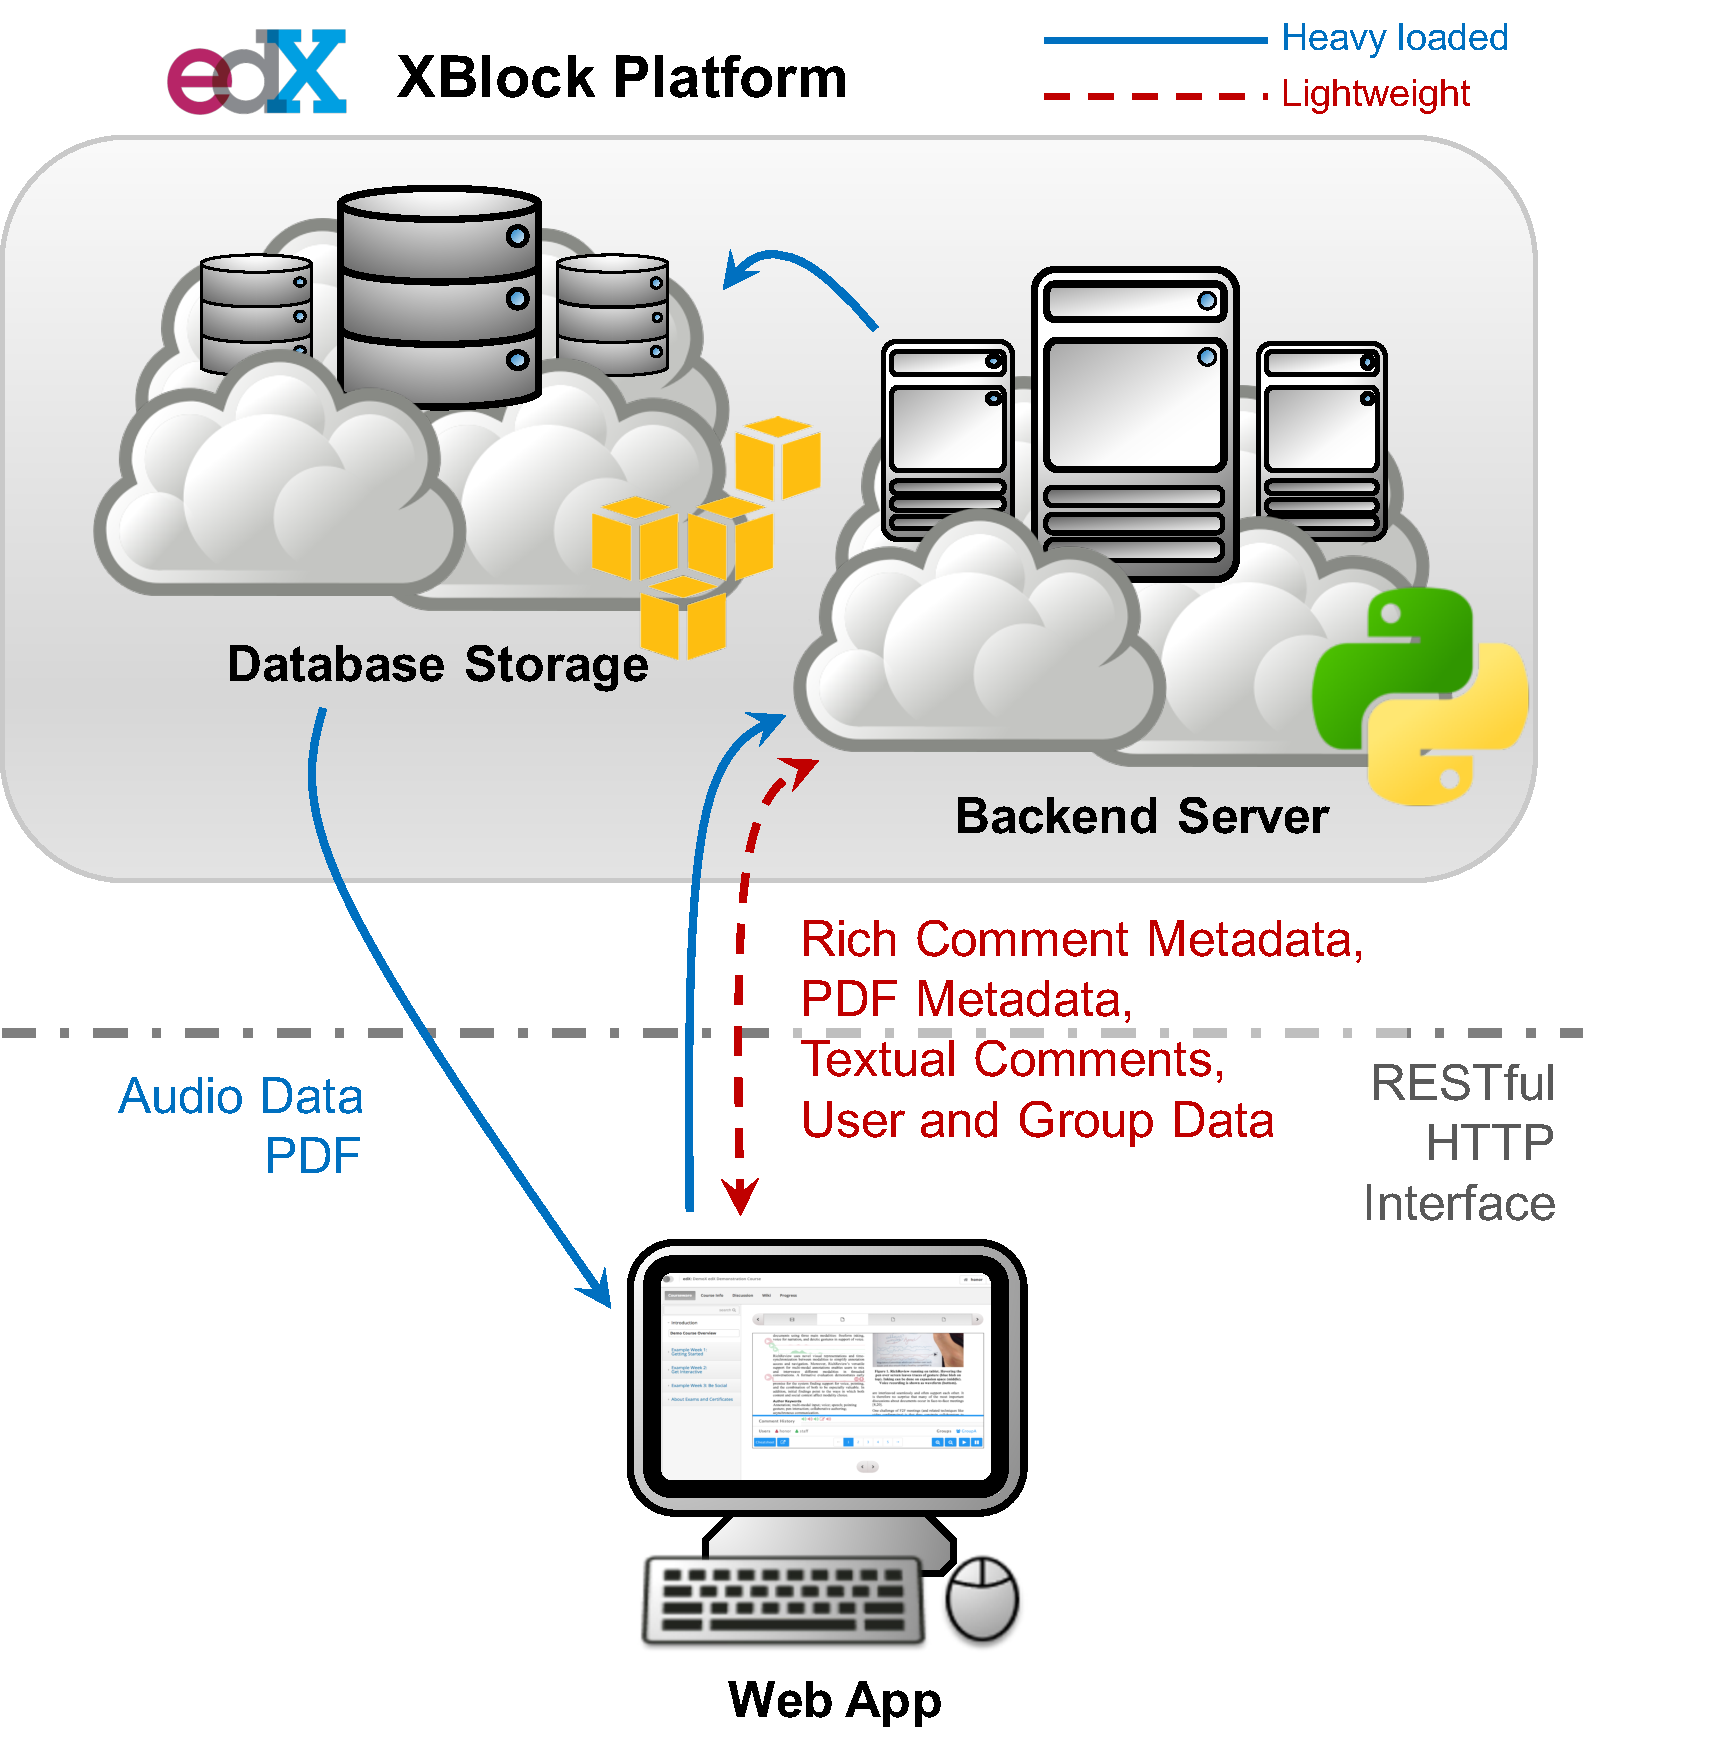
\includegraphics[width=0.95\columnwidth]{figure_architecture}
\caption{Scalable back-end architecture of the multimodal annotation system.}
\label{fig:scalable}
\end{figure}

\section{Integration into edX.org} 

In prior work, we saw RichReview perform well in traditional classroom settings~cite{something-or-other}. 
In order to more accurately measure the impact of RichReview, we would like to integrate it into a setting which supports massive numbers of learners. 
Open edX is a platform which support both MOOCs, with millions of learners on the edx.org web site, a large level of residential use (over 80\% of MIT students use edX residentially), over 100 open source deployments, including several deployments as part of national initiatives to improve training and education.
Open edX was chosen due to the combination of support for research (including frameworks for randomized control trials, data collection, and frameworks for integration with novel pedagogical experiences like RichReview), anecdotal data from residential trials, and statistical evidence from MOOC trials. 

A key to success is seamless integration into the platform, including support for scaling to tens of thousands of learners. As part of bringing RichReview to scale, we re-implemented the RichReview system as an XBlock -- the components out of which Open edX courses are built.
This allows the MOOC authors to include RichReview discussion sessions without managing multiple services, and for MOOC students to use the compenent seamlessly integrated into the edX interface.
As can be seen in Fig.~\ref{fig:screenshot}, the instructor can place the RichReview discussion session within the flow of the course contents. The overall system architecture is shown in Fig.~\ref{fig:scalable}

\subsection{Making the Back-end Scalable}
RichReview is a media-heavy web application that exchanges large amounts of audio-visual data with the server.
With tens of thousands of learners, designing a scalable back-end architecture of RichReview is essential to successful deployment.
We broke the data elements of RichReview into the two types: heavy-load multimedia data such as audio recording and PDF documents, and lightweight metadata including textual notes and audio meta information.
The heavy-weight components are distributed through cloud file storage --- in our case, Amazon Simple Storage Service (S3) --- which gives complete horizontal scalability. The metadata and other small data live in a conventional database. This allows queries for rapid access to many pieces of metadata.

\subsection{Semantic Voice Editing}
From our prior RichReview deployment study~\cite{yoon2015richreview}, the discussant sometimes had to re-record an entire voice interaction to fix small mistakes in the middle of the recording, such as a stutter or a long pause.
Recently, Rubin et al. presented an audio editing system that leverages speech transcriptions as semantic guidelines for editing voice as if it is text \cite{rubin2013content}.
We are following this semantic editing approach, focusing on design and development of live editing features, such as partial deletion or insertion.
Even after having the caption-based editing system, it is a tedious repetitive task to manually trim long-pauses and 'Um's~\cite{yoon2014richreview}.
We will solve this problem by providing a batch post-processing operation that can automatically delete several such unnecessary snippets at once.

\subsection{Profile Based Group-assignment}
Assigning students to groups that can maximize overall diversity of the member compositions.

\section{Acknowledgement} 
Dongwook Yoon gratefully acknowledges the support from the Kwanjeong educational foundation.

\bibliographystyle{acm-sigchi}
\bibliography{sample}
\end{document}
